\documentclass[twoside]{book}

% Packages required by doxygen
\usepackage{fixltx2e}
\usepackage{calc}
\usepackage{doxygen}
\usepackage[export]{adjustbox} % also loads graphicx
\usepackage{graphicx}
\usepackage[utf8]{inputenc}
\usepackage{makeidx}
\usepackage{multicol}
\usepackage{multirow}
\PassOptionsToPackage{warn}{textcomp}
\usepackage{textcomp}
\usepackage[nointegrals]{wasysym}
\usepackage[table]{xcolor}

% Font selection
\usepackage[T1]{fontenc}
\usepackage[scaled=.90]{helvet}
\usepackage{courier}
\usepackage{amssymb}
\usepackage{sectsty}
\renewcommand{\familydefault}{\sfdefault}
\allsectionsfont{%
  \fontseries{bc}\selectfont%
  \color{darkgray}%
}
\renewcommand{\DoxyLabelFont}{%
  \fontseries{bc}\selectfont%
  \color{darkgray}%
}
\newcommand{\+}{\discretionary{\mbox{\scriptsize$\hookleftarrow$}}{}{}}

% Page & text layout
\usepackage{geometry}
\geometry{%
  a4paper,%
  top=2.5cm,%
  bottom=2.5cm,%
  left=2.5cm,%
  right=2.5cm%
}
\tolerance=750
\hfuzz=15pt
\hbadness=750
\setlength{\emergencystretch}{15pt}
\setlength{\parindent}{0cm}
\setlength{\parskip}{0.2cm}
\makeatletter
\renewcommand{\paragraph}{%
  \@startsection{paragraph}{4}{0ex}{-1.0ex}{1.0ex}{%
    \normalfont\normalsize\bfseries\SS@parafont%
  }%
}
\renewcommand{\subparagraph}{%
  \@startsection{subparagraph}{5}{0ex}{-1.0ex}{1.0ex}{%
    \normalfont\normalsize\bfseries\SS@subparafont%
  }%
}
\makeatother

% Headers & footers
\usepackage{fancyhdr}
\pagestyle{fancyplain}
\fancyhead[LE]{\fancyplain{}{\bfseries\thepage}}
\fancyhead[CE]{\fancyplain{}{}}
\fancyhead[RE]{\fancyplain{}{\bfseries\leftmark}}
\fancyhead[LO]{\fancyplain{}{\bfseries\rightmark}}
\fancyhead[CO]{\fancyplain{}{}}
\fancyhead[RO]{\fancyplain{}{\bfseries\thepage}}
\fancyfoot[LE]{\fancyplain{}{}}
\fancyfoot[CE]{\fancyplain{}{}}
\fancyfoot[RE]{\fancyplain{}{\bfseries\scriptsize Generated on Sun Nov 15 2015 17\+:16\+:19 for invest\+\_\+doxygen by Doxygen }}
\fancyfoot[LO]{\fancyplain{}{\bfseries\scriptsize Generated on Sun Nov 15 2015 17\+:16\+:19 for invest\+\_\+doxygen by Doxygen }}
\fancyfoot[CO]{\fancyplain{}{}}
\fancyfoot[RO]{\fancyplain{}{}}
\renewcommand{\footrulewidth}{0.4pt}
\renewcommand{\chaptermark}[1]{%
  \markboth{#1}{}%
}
\renewcommand{\sectionmark}[1]{%
  \markright{\thesection\ #1}%
}

% Indices & bibliography
\usepackage{natbib}
\usepackage[titles]{tocloft}
\setcounter{tocdepth}{3}
\setcounter{secnumdepth}{5}
\makeindex

% Hyperlinks (required, but should be loaded last)
\usepackage{ifpdf}
\ifpdf
  \usepackage[pdftex,pagebackref=true]{hyperref}
\else
  \usepackage[ps2pdf,pagebackref=true]{hyperref}
\fi
\hypersetup{%
  colorlinks=true,%
  linkcolor=blue,%
  citecolor=blue,%
  unicode%
}

% Custom commands
\newcommand{\clearemptydoublepage}{%
  \newpage{\pagestyle{empty}\cleardoublepage}%
}


%===== C O N T E N T S =====

\begin{document}

% Titlepage & ToC
\hypersetup{pageanchor=false,
             bookmarks=true,
             bookmarksnumbered=true,
             pdfencoding=unicode
            }
\pagenumbering{roman}
\begin{titlepage}
\vspace*{7cm}
\begin{center}%
{\Large invest\+\_\+doxygen }\\
\vspace*{1cm}
{\large Generated by Doxygen 1.8.10}\\
\vspace*{0.5cm}
{\small Sun Nov 15 2015 17:16:19}\\
\end{center}
\end{titlepage}
\clearemptydoublepage
\tableofcontents
\clearemptydoublepage
\pagenumbering{arabic}
\hypersetup{pageanchor=true}

%--- Begin generated contents ---
\chapter{Main Page}
\label{index}\hypertarget{index}{}\hyperlink{main_8cpp}{main.\+cpp} assign2\+\_\+prototype

Created by Dustin on 2015-\/11-\/11. Copyright © 2015 Dustin. All rights reserved. 
\chapter{Hierarchical Index}
\section{Class Hierarchy}
This inheritance list is sorted roughly, but not completely, alphabetically\+:\begin{DoxyCompactList}
\item \contentsline{section}{Index}{\pageref{class_index}}{}
\begin{DoxyCompactList}
\item \contentsline{section}{Mutual\+Fund}{\pageref{class_mutual_fund}}{}
\item \contentsline{section}{Stock}{\pageref{class_stock}}{}
\end{DoxyCompactList}
\item Message\begin{DoxyCompactList}
\item \contentsline{section}{invest\+:\+:Investment}{\pageref{classinvest_1_1_investment}}{}
\item \contentsline{section}{invest\+:\+:Portfolio}{\pageref{classinvest_1_1_portfolio}}{}
\end{DoxyCompactList}
\item \contentsline{section}{Obj\+Factory}{\pageref{class_obj_factory}}{}
\item \contentsline{section}{invest\+:\+:Static\+Descriptor\+Initializer\+\_\+invest\+\_\+2eproto}{\pageref{structinvest_1_1_static_descriptor_initializer__invest__2eproto}}{}
\end{DoxyCompactList}

\chapter{Class Index}
\section{Class List}
Here are the classes, structs, unions and interfaces with brief descriptions\+:\begin{DoxyCompactList}
\item\contentsline{section}{\hyperlink{class_index}{Index} }{\pageref{class_index}}{}
\item\contentsline{section}{\hyperlink{classinvest_1_1_investment}{invest\+::\+Investment} }{\pageref{classinvest_1_1_investment}}{}
\item\contentsline{section}{\hyperlink{class_mutual_fund}{Mutual\+Fund} }{\pageref{class_mutual_fund}}{}
\item\contentsline{section}{\hyperlink{class_obj_factory}{Obj\+Factory} }{\pageref{class_obj_factory}}{}
\item\contentsline{section}{\hyperlink{classinvest_1_1_portfolio}{invest\+::\+Portfolio} }{\pageref{classinvest_1_1_portfolio}}{}
\item\contentsline{section}{\hyperlink{structinvest_1_1_static_descriptor_initializer__invest__2eproto}{invest\+::\+Static\+Descriptor\+Initializer\+\_\+invest\+\_\+2eproto} }{\pageref{structinvest_1_1_static_descriptor_initializer__invest__2eproto}}{}
\item\contentsline{section}{\hyperlink{class_stock}{Stock} }{\pageref{class_stock}}{}
\end{DoxyCompactList}

\chapter{File Index}
\section{File List}
Here is a list of all files with brief descriptions\+:\begin{DoxyCompactList}
\item\contentsline{section}{/\+Users/dustin/\+Documents/\+Seng330\+\_\+\+Assign2/assign2\+\_\+prototype/assign2\+\_\+prototype/\hyperlink{main_8cpp}{main.\+cpp} }{\pageref{main_8cpp}}{}
\end{DoxyCompactList}

\chapter{Class Documentation}
\hypertarget{class_base}{}\section{Base Class Reference}
\label{class_base}\index{Base@{Base}}
Inheritance diagram for Base\+:\begin{figure}[H]
\begin{center}
\leavevmode
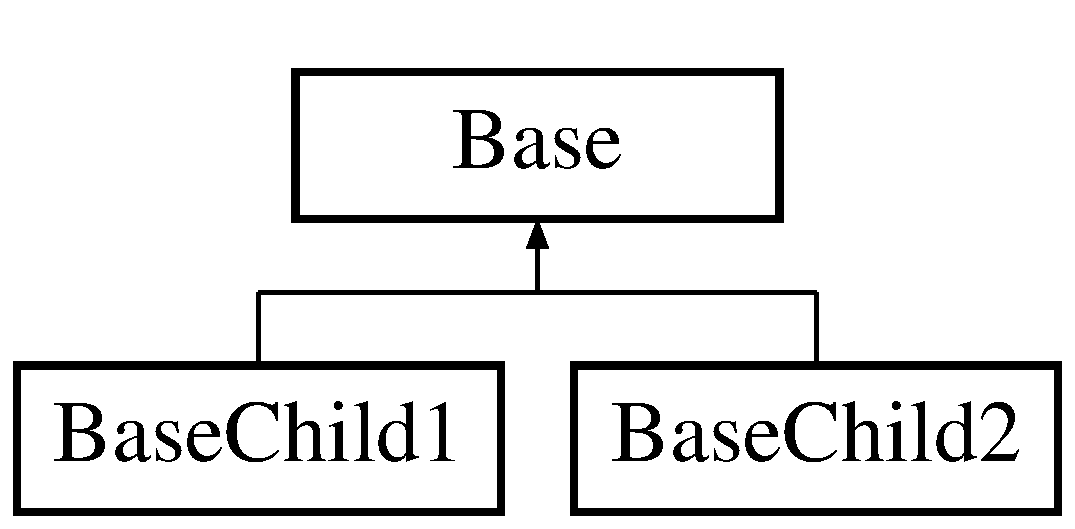
\includegraphics[height=2.000000cm]{class_base}
\end{center}
\end{figure}
\subsection*{Public Member Functions}
\begin{DoxyCompactItemize}
\item 
virtual \hyperlink{class_base}{Base} $\ast$ \hyperlink{class_base_a7af9a54603d875a8195502c21aab84f0}{clone} ()=0
\item 
string \hyperlink{class_base_a27e9a4dfa1de26371837b83d2570f856}{get\+C\+Name} ()
\end{DoxyCompactItemize}
\subsection*{Protected Attributes}
\begin{DoxyCompactItemize}
\item 
string \hyperlink{class_base_a4e9d36a510c93b909535c8b91d1b006e}{cname}
\end{DoxyCompactItemize}


\subsection{Detailed Description}
This is the \hyperlink{class_base}{Base} Prototype class that will be the template for other classes 

\subsection{Member Function Documentation}
\hypertarget{class_base_a7af9a54603d875a8195502c21aab84f0}{}\index{Base@{Base}!clone@{clone}}
\index{clone@{clone}!Base@{Base}}
\subsubsection[{clone()=0}]{\setlength{\rightskip}{0pt plus 5cm}virtual {\bf Base}$\ast$ Base\+::clone (
\begin{DoxyParamCaption}
{}
\end{DoxyParamCaption}
)\hspace{0.3cm}{\ttfamily [pure virtual]}}\label{class_base_a7af9a54603d875a8195502c21aab84f0}
Template for clone 

Implemented in \hyperlink{class_base_child2_aa9d76ba1f050d535f432ff663995394a}{Base\+Child2}, and \hyperlink{class_base_child1_ab88f5812145b6d015e47b8edb781f8a5}{Base\+Child1}.

\hypertarget{class_base_a27e9a4dfa1de26371837b83d2570f856}{}\index{Base@{Base}!get\+C\+Name@{get\+C\+Name}}
\index{get\+C\+Name@{get\+C\+Name}!Base@{Base}}
\subsubsection[{get\+C\+Name()}]{\setlength{\rightskip}{0pt plus 5cm}string Base\+::get\+C\+Name (
\begin{DoxyParamCaption}
{}
\end{DoxyParamCaption}
)\hspace{0.3cm}{\ttfamily [inline]}}\label{class_base_a27e9a4dfa1de26371837b83d2570f856}
Getter method for cname 

\subsection{Member Data Documentation}
\hypertarget{class_base_a4e9d36a510c93b909535c8b91d1b006e}{}\index{Base@{Base}!cname@{cname}}
\index{cname@{cname}!Base@{Base}}
\subsubsection[{cname}]{\setlength{\rightskip}{0pt plus 5cm}string Base\+::cname\hspace{0.3cm}{\ttfamily [protected]}}\label{class_base_a4e9d36a510c93b909535c8b91d1b006e}
Protected string cname 

The documentation for this class was generated from the following file\+:\begin{DoxyCompactItemize}
\item 
/\+Users/dustin/\+Documents/\+Seng330\+\_\+\+Assign2/assign2\+\_\+prototype/assign2\+\_\+prototype/\hyperlink{main_8cpp}{main.\+cpp}\end{DoxyCompactItemize}

\hypertarget{class_base_child1}{}\section{Base\+Child1 Class Reference}
\label{class_base_child1}\index{Base\+Child1@{Base\+Child1}}
Inheritance diagram for Base\+Child1\+:\begin{figure}[H]
\begin{center}
\leavevmode
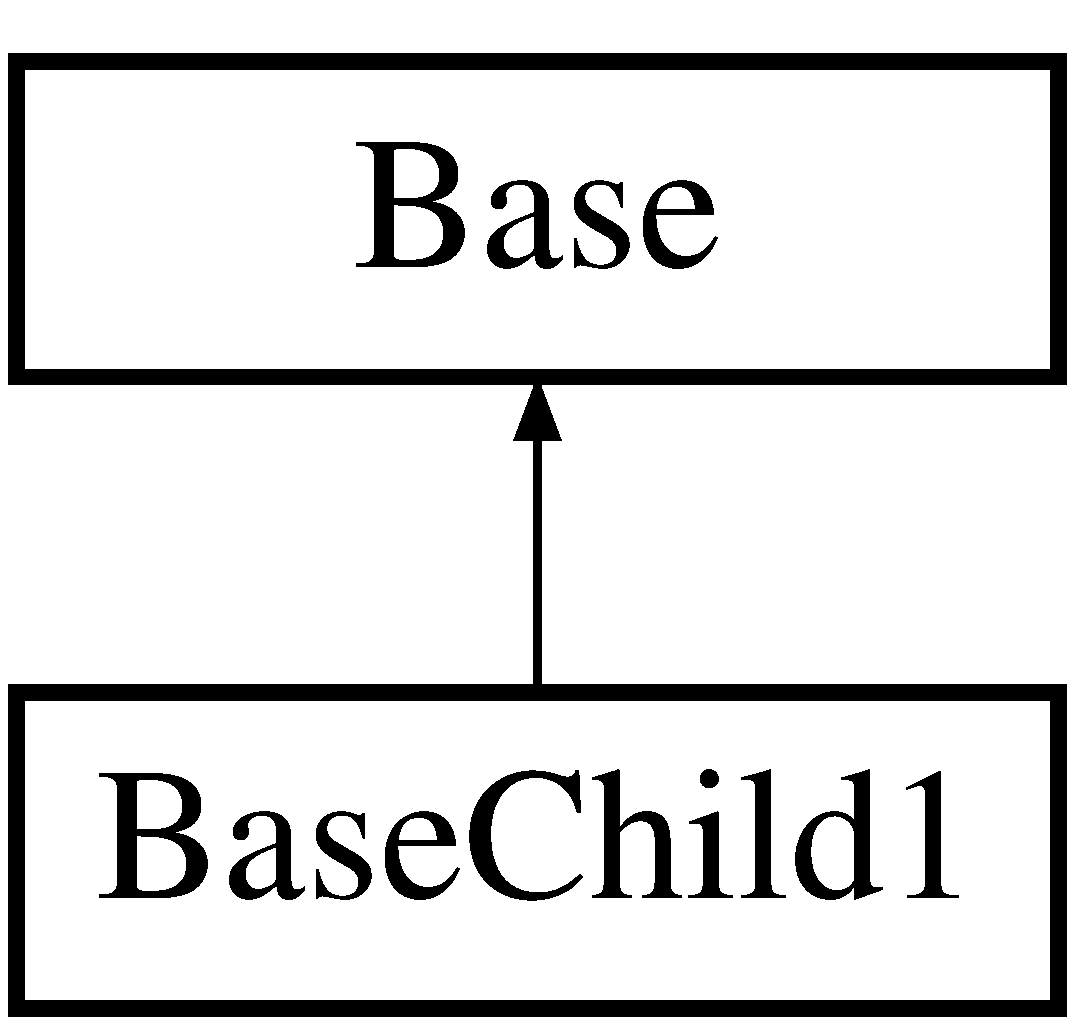
\includegraphics[height=2.000000cm]{class_base_child1}
\end{center}
\end{figure}
\subsection*{Public Member Functions}
\begin{DoxyCompactItemize}
\item 
\hyperlink{class_base_child1_a7b0715b89a69ea3fb193512296af8a87}{Base\+Child1} (string str)
\item 
\hyperlink{class_base}{Base} $\ast$ \hyperlink{class_base_child1_ab88f5812145b6d015e47b8edb781f8a5}{clone} ()
\item 
\hyperlink{class_base_child1_a4dd7fe56f7d46e826e940ea908fec468}{$\sim$\+Base\+Child1} ()
\end{DoxyCompactItemize}
\subsection*{Additional Inherited Members}


\subsection{Detailed Description}
This is the Stock Prototype class that will be the template to be cloned for a stock 

\subsection{Constructor \& Destructor Documentation}
\hypertarget{class_base_child1_a7b0715b89a69ea3fb193512296af8a87}{}\index{Base\+Child1@{Base\+Child1}!Base\+Child1@{Base\+Child1}}
\index{Base\+Child1@{Base\+Child1}!Base\+Child1@{Base\+Child1}}
\subsubsection[{Base\+Child1(string str)}]{\setlength{\rightskip}{0pt plus 5cm}Base\+Child1\+::\+Base\+Child1 (
\begin{DoxyParamCaption}
\item[{string}]{str}
\end{DoxyParamCaption}
)\hspace{0.3cm}{\ttfamily [inline]}}\label{class_base_child1_a7b0715b89a69ea3fb193512296af8a87}
Constructor for \hyperlink{class_base_child1}{Base\+Child1} with string value \hypertarget{class_base_child1_a4dd7fe56f7d46e826e940ea908fec468}{}\index{Base\+Child1@{Base\+Child1}!````~Base\+Child1@{$\sim$\+Base\+Child1}}
\index{````~Base\+Child1@{$\sim$\+Base\+Child1}!Base\+Child1@{Base\+Child1}}
\subsubsection[{$\sim$\+Base\+Child1()}]{\setlength{\rightskip}{0pt plus 5cm}Base\+Child1\+::$\sim$\+Base\+Child1 (
\begin{DoxyParamCaption}
{}
\end{DoxyParamCaption}
)\hspace{0.3cm}{\ttfamily [inline]}}\label{class_base_child1_a4dd7fe56f7d46e826e940ea908fec468}
Destructor function for \hyperlink{class_base_child1}{Base\+Child1} 

\subsection{Member Function Documentation}
\hypertarget{class_base_child1_ab88f5812145b6d015e47b8edb781f8a5}{}\index{Base\+Child1@{Base\+Child1}!clone@{clone}}
\index{clone@{clone}!Base\+Child1@{Base\+Child1}}
\subsubsection[{clone()}]{\setlength{\rightskip}{0pt plus 5cm}{\bf Base}$\ast$ Base\+Child1\+::clone (
\begin{DoxyParamCaption}
{}
\end{DoxyParamCaption}
)\hspace{0.3cm}{\ttfamily [inline]}, {\ttfamily [virtual]}}\label{class_base_child1_ab88f5812145b6d015e47b8edb781f8a5}
Clone function for \hyperlink{class_base_child1}{Base\+Child1} 

Implements \hyperlink{class_base_a7af9a54603d875a8195502c21aab84f0}{Base}.



The documentation for this class was generated from the following file\+:\begin{DoxyCompactItemize}
\item 
/\+Users/dustin/\+Documents/\+Seng330\+\_\+\+Assign2/assign2\+\_\+prototype/assign2\+\_\+prototype/\hyperlink{main_8cpp}{main.\+cpp}\end{DoxyCompactItemize}

\hypertarget{class_base_child2}{}\section{Base\+Child2 Class Reference}
\label{class_base_child2}\index{Base\+Child2@{Base\+Child2}}
Inheritance diagram for Base\+Child2\+:\begin{figure}[H]
\begin{center}
\leavevmode
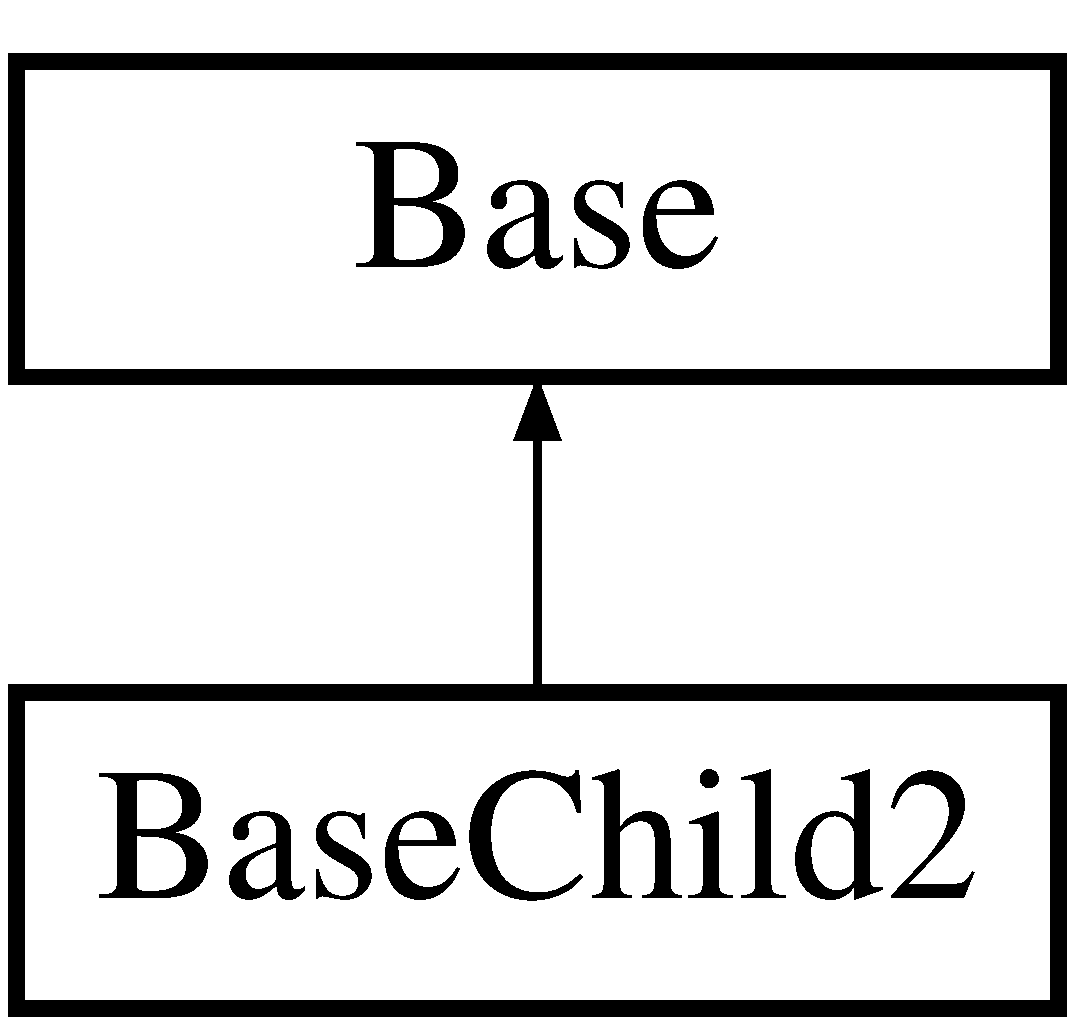
\includegraphics[height=2.000000cm]{class_base_child2}
\end{center}
\end{figure}
\subsection*{Public Member Functions}
\begin{DoxyCompactItemize}
\item 
\hyperlink{class_base_child2_ab6cf6f80a1e1f5aff15a3b7e2b646c21}{Base\+Child2} (string str)
\item 
\hyperlink{class_base}{Base} $\ast$ \hyperlink{class_base_child2_aa9d76ba1f050d535f432ff663995394a}{clone} ()
\item 
\hyperlink{class_base_child2_afecb5170de396eb42b889dfd3acd489b}{$\sim$\+Base\+Child2} ()
\end{DoxyCompactItemize}
\subsection*{Additional Inherited Members}


\subsection{Detailed Description}
This is the Mutual\+Fund Prototype class that will be the template to be cloned for a Mutual\+Fund 

\subsection{Constructor \& Destructor Documentation}
\hypertarget{class_base_child2_ab6cf6f80a1e1f5aff15a3b7e2b646c21}{}\index{Base\+Child2@{Base\+Child2}!Base\+Child2@{Base\+Child2}}
\index{Base\+Child2@{Base\+Child2}!Base\+Child2@{Base\+Child2}}
\subsubsection[{Base\+Child2(string str)}]{\setlength{\rightskip}{0pt plus 5cm}Base\+Child2\+::\+Base\+Child2 (
\begin{DoxyParamCaption}
\item[{string}]{str}
\end{DoxyParamCaption}
)\hspace{0.3cm}{\ttfamily [inline]}}\label{class_base_child2_ab6cf6f80a1e1f5aff15a3b7e2b646c21}
Constructor for \hyperlink{class_base_child2}{Base\+Child2} with string value \hypertarget{class_base_child2_afecb5170de396eb42b889dfd3acd489b}{}\index{Base\+Child2@{Base\+Child2}!````~Base\+Child2@{$\sim$\+Base\+Child2}}
\index{````~Base\+Child2@{$\sim$\+Base\+Child2}!Base\+Child2@{Base\+Child2}}
\subsubsection[{$\sim$\+Base\+Child2()}]{\setlength{\rightskip}{0pt plus 5cm}Base\+Child2\+::$\sim$\+Base\+Child2 (
\begin{DoxyParamCaption}
{}
\end{DoxyParamCaption}
)\hspace{0.3cm}{\ttfamily [inline]}}\label{class_base_child2_afecb5170de396eb42b889dfd3acd489b}
Destructor function for \hyperlink{class_base_child2}{Base\+Child2} 

\subsection{Member Function Documentation}
\hypertarget{class_base_child2_aa9d76ba1f050d535f432ff663995394a}{}\index{Base\+Child2@{Base\+Child2}!clone@{clone}}
\index{clone@{clone}!Base\+Child2@{Base\+Child2}}
\subsubsection[{clone()}]{\setlength{\rightskip}{0pt plus 5cm}{\bf Base}$\ast$ Base\+Child2\+::clone (
\begin{DoxyParamCaption}
{}
\end{DoxyParamCaption}
)\hspace{0.3cm}{\ttfamily [inline]}, {\ttfamily [virtual]}}\label{class_base_child2_aa9d76ba1f050d535f432ff663995394a}
Clone function for \hyperlink{class_base_child2}{Base\+Child2} 

Implements \hyperlink{class_base_a7af9a54603d875a8195502c21aab84f0}{Base}.



The documentation for this class was generated from the following file\+:\begin{DoxyCompactItemize}
\item 
/\+Users/dustin/\+Documents/\+Seng330\+\_\+\+Assign2/assign2\+\_\+prototype/assign2\+\_\+prototype/\hyperlink{main_8cpp}{main.\+cpp}\end{DoxyCompactItemize}

\hypertarget{class_obj_factory}{}\section{Obj\+Factory Class Reference}
\label{class_obj_factory}\index{Obj\+Factory@{Obj\+Factory}}
\subsection*{Static Public Member Functions}
\begin{DoxyCompactItemize}
\item 
static void \hyperlink{class_obj_factory_a0b98b0d414dd16735397434d42060db0}{init} ()
\item 
static \hyperlink{class_index}{Index} $\ast$ \hyperlink{class_obj_factory_aba4ecb86a449ca141e374ceee8a67077}{get\+Name\+Val1} ()
\item 
static \hyperlink{class_index}{Index} $\ast$ \hyperlink{class_obj_factory_a18f359e3e70223f815c9cbc3ce0e036e}{get\+Name\+Val2} ()
\end{DoxyCompactItemize}


\subsection{Member Function Documentation}
\hypertarget{class_obj_factory_aba4ecb86a449ca141e374ceee8a67077}{}\index{Obj\+Factory@{Obj\+Factory}!get\+Name\+Val1@{get\+Name\+Val1}}
\index{get\+Name\+Val1@{get\+Name\+Val1}!Obj\+Factory@{Obj\+Factory}}
\subsubsection[{get\+Name\+Val1()}]{\setlength{\rightskip}{0pt plus 5cm}static {\bf Index}$\ast$ Obj\+Factory\+::get\+Name\+Val1 (
\begin{DoxyParamCaption}
{}
\end{DoxyParamCaption}
)\hspace{0.3cm}{\ttfamily [inline]}, {\ttfamily [static]}}\label{class_obj_factory_aba4ecb86a449ca141e374ceee8a67077}
Function to clone derived class 1 \hypertarget{class_obj_factory_a18f359e3e70223f815c9cbc3ce0e036e}{}\index{Obj\+Factory@{Obj\+Factory}!get\+Name\+Val2@{get\+Name\+Val2}}
\index{get\+Name\+Val2@{get\+Name\+Val2}!Obj\+Factory@{Obj\+Factory}}
\subsubsection[{get\+Name\+Val2()}]{\setlength{\rightskip}{0pt plus 5cm}static {\bf Index}$\ast$ Obj\+Factory\+::get\+Name\+Val2 (
\begin{DoxyParamCaption}
{}
\end{DoxyParamCaption}
)\hspace{0.3cm}{\ttfamily [inline]}, {\ttfamily [static]}}\label{class_obj_factory_a18f359e3e70223f815c9cbc3ce0e036e}
Function to clone derived class 2 \hypertarget{class_obj_factory_a0b98b0d414dd16735397434d42060db0}{}\index{Obj\+Factory@{Obj\+Factory}!init@{init}}
\index{init@{init}!Obj\+Factory@{Obj\+Factory}}
\subsubsection[{init()}]{\setlength{\rightskip}{0pt plus 5cm}static void Obj\+Factory\+::init (
\begin{DoxyParamCaption}
{}
\end{DoxyParamCaption}
)\hspace{0.3cm}{\ttfamily [inline]}, {\ttfamily [static]}}\label{class_obj_factory_a0b98b0d414dd16735397434d42060db0}
Initialization function of derived classes 

The documentation for this class was generated from the following file\+:\begin{DoxyCompactItemize}
\item 
/\+Users/dustin/\+Documents/\+Seng330\+\_\+\+Assign2/src/\hyperlink{main_8cpp}{main.\+cpp}\end{DoxyCompactItemize}

\chapter{File Documentation}
\hypertarget{main_8cpp}{}\section{/\+Users/dustin/\+Documents/\+Seng330\+\_\+\+Assign2/assign2\+\_\+prototype/assign2\+\_\+prototype/main.cpp File Reference}
\label{main_8cpp}\index{/\+Users/dustin/\+Documents/\+Seng330\+\_\+\+Assign2/assign2\+\_\+prototype/assign2\+\_\+prototype/main.\+cpp@{/\+Users/dustin/\+Documents/\+Seng330\+\_\+\+Assign2/assign2\+\_\+prototype/assign2\+\_\+prototype/main.\+cpp}}
{\ttfamily \#include $<$iostream$>$}\\*
{\ttfamily \#include $<$string$>$}\\*
\subsection*{Classes}
\begin{DoxyCompactItemize}
\item 
class \hyperlink{class_base}{Base}
\item 
class \hyperlink{class_base_child1}{Base\+Child1}
\item 
class \hyperlink{class_base_child2}{Base\+Child2}
\item 
class \hyperlink{class_obj_factory}{Obj\+Factory}
\end{DoxyCompactItemize}
\subsection*{Functions}
\begin{DoxyCompactItemize}
\item 
int \hyperlink{main_8cpp_ac0f2228420376f4db7e1274f2b41667c}{main} (int argc, const char $\ast$argv\mbox{[}$\,$\mbox{]})
\end{DoxyCompactItemize}


\subsection{Function Documentation}
\hypertarget{main_8cpp_ac0f2228420376f4db7e1274f2b41667c}{}\index{main.\+cpp@{main.\+cpp}!main@{main}}
\index{main@{main}!main.\+cpp@{main.\+cpp}}
\subsubsection[{main(int argc, const char $\ast$argv[])}]{\setlength{\rightskip}{0pt plus 5cm}int main (
\begin{DoxyParamCaption}
\item[{int}]{argc, }
\item[{const char $\ast$}]{argv\mbox{[}$\,$\mbox{]}}
\end{DoxyParamCaption}
)}\label{main_8cpp_ac0f2228420376f4db7e1274f2b41667c}
Main function for execution of creating classes and producing objects from user interaction. There is a \hyperlink{class_base}{Base} class that acts as a template and two derived classes Stock and Mutual\+Fund. Initialization of Objects and variables
%--- End generated contents ---

% Index
\backmatter
\newpage
\phantomsection
\clearemptydoublepage
\addcontentsline{toc}{chapter}{Index}
\printindex

\end{document}
